% Options for packages loaded elsewhere
\PassOptionsToPackage{unicode}{hyperref}
\PassOptionsToPackage{hyphens}{url}
%
\documentclass[
]{article}
\usepackage{amsmath,amssymb}
\usepackage{lmodern}
\usepackage{ifxetex,ifluatex}
\ifnum 0\ifxetex 1\fi\ifluatex 1\fi=0 % if pdftex
  \usepackage[T1]{fontenc}
  \usepackage[utf8]{inputenc}
  \usepackage{textcomp} % provide euro and other symbols
\else % if luatex or xetex
  \usepackage{unicode-math}
  \defaultfontfeatures{Scale=MatchLowercase}
  \defaultfontfeatures[\rmfamily]{Ligatures=TeX,Scale=1}
\fi
% Use upquote if available, for straight quotes in verbatim environments
\IfFileExists{upquote.sty}{\usepackage{upquote}}{}
\IfFileExists{microtype.sty}{% use microtype if available
  \usepackage[]{microtype}
  \UseMicrotypeSet[protrusion]{basicmath} % disable protrusion for tt fonts
}{}
\makeatletter
\@ifundefined{KOMAClassName}{% if non-KOMA class
  \IfFileExists{parskip.sty}{%
    \usepackage{parskip}
  }{% else
    \setlength{\parindent}{0pt}
    \setlength{\parskip}{6pt plus 2pt minus 1pt}}
}{% if KOMA class
  \KOMAoptions{parskip=half}}
\makeatother
\usepackage{xcolor}
\IfFileExists{xurl.sty}{\usepackage{xurl}}{} % add URL line breaks if available
\IfFileExists{bookmark.sty}{\usepackage{bookmark}}{\usepackage{hyperref}}
\hypersetup{
  pdftitle={cluster jerarquico en R},
  pdfauthor={Jaime Isaac},
  hidelinks,
  pdfcreator={LaTeX via pandoc}}
\urlstyle{same} % disable monospaced font for URLs
\usepackage[margin=1in]{geometry}
\usepackage{color}
\usepackage{fancyvrb}
\newcommand{\VerbBar}{|}
\newcommand{\VERB}{\Verb[commandchars=\\\{\}]}
\DefineVerbatimEnvironment{Highlighting}{Verbatim}{commandchars=\\\{\}}
% Add ',fontsize=\small' for more characters per line
\usepackage{framed}
\definecolor{shadecolor}{RGB}{248,248,248}
\newenvironment{Shaded}{\begin{snugshade}}{\end{snugshade}}
\newcommand{\AlertTok}[1]{\textcolor[rgb]{0.94,0.16,0.16}{#1}}
\newcommand{\AnnotationTok}[1]{\textcolor[rgb]{0.56,0.35,0.01}{\textbf{\textit{#1}}}}
\newcommand{\AttributeTok}[1]{\textcolor[rgb]{0.77,0.63,0.00}{#1}}
\newcommand{\BaseNTok}[1]{\textcolor[rgb]{0.00,0.00,0.81}{#1}}
\newcommand{\BuiltInTok}[1]{#1}
\newcommand{\CharTok}[1]{\textcolor[rgb]{0.31,0.60,0.02}{#1}}
\newcommand{\CommentTok}[1]{\textcolor[rgb]{0.56,0.35,0.01}{\textit{#1}}}
\newcommand{\CommentVarTok}[1]{\textcolor[rgb]{0.56,0.35,0.01}{\textbf{\textit{#1}}}}
\newcommand{\ConstantTok}[1]{\textcolor[rgb]{0.00,0.00,0.00}{#1}}
\newcommand{\ControlFlowTok}[1]{\textcolor[rgb]{0.13,0.29,0.53}{\textbf{#1}}}
\newcommand{\DataTypeTok}[1]{\textcolor[rgb]{0.13,0.29,0.53}{#1}}
\newcommand{\DecValTok}[1]{\textcolor[rgb]{0.00,0.00,0.81}{#1}}
\newcommand{\DocumentationTok}[1]{\textcolor[rgb]{0.56,0.35,0.01}{\textbf{\textit{#1}}}}
\newcommand{\ErrorTok}[1]{\textcolor[rgb]{0.64,0.00,0.00}{\textbf{#1}}}
\newcommand{\ExtensionTok}[1]{#1}
\newcommand{\FloatTok}[1]{\textcolor[rgb]{0.00,0.00,0.81}{#1}}
\newcommand{\FunctionTok}[1]{\textcolor[rgb]{0.00,0.00,0.00}{#1}}
\newcommand{\ImportTok}[1]{#1}
\newcommand{\InformationTok}[1]{\textcolor[rgb]{0.56,0.35,0.01}{\textbf{\textit{#1}}}}
\newcommand{\KeywordTok}[1]{\textcolor[rgb]{0.13,0.29,0.53}{\textbf{#1}}}
\newcommand{\NormalTok}[1]{#1}
\newcommand{\OperatorTok}[1]{\textcolor[rgb]{0.81,0.36,0.00}{\textbf{#1}}}
\newcommand{\OtherTok}[1]{\textcolor[rgb]{0.56,0.35,0.01}{#1}}
\newcommand{\PreprocessorTok}[1]{\textcolor[rgb]{0.56,0.35,0.01}{\textit{#1}}}
\newcommand{\RegionMarkerTok}[1]{#1}
\newcommand{\SpecialCharTok}[1]{\textcolor[rgb]{0.00,0.00,0.00}{#1}}
\newcommand{\SpecialStringTok}[1]{\textcolor[rgb]{0.31,0.60,0.02}{#1}}
\newcommand{\StringTok}[1]{\textcolor[rgb]{0.31,0.60,0.02}{#1}}
\newcommand{\VariableTok}[1]{\textcolor[rgb]{0.00,0.00,0.00}{#1}}
\newcommand{\VerbatimStringTok}[1]{\textcolor[rgb]{0.31,0.60,0.02}{#1}}
\newcommand{\WarningTok}[1]{\textcolor[rgb]{0.56,0.35,0.01}{\textbf{\textit{#1}}}}
\usepackage{graphicx}
\makeatletter
\def\maxwidth{\ifdim\Gin@nat@width>\linewidth\linewidth\else\Gin@nat@width\fi}
\def\maxheight{\ifdim\Gin@nat@height>\textheight\textheight\else\Gin@nat@height\fi}
\makeatother
% Scale images if necessary, so that they will not overflow the page
% margins by default, and it is still possible to overwrite the defaults
% using explicit options in \includegraphics[width, height, ...]{}
\setkeys{Gin}{width=\maxwidth,height=\maxheight,keepaspectratio}
% Set default figure placement to htbp
\makeatletter
\def\fps@figure{htbp}
\makeatother
\setlength{\emergencystretch}{3em} % prevent overfull lines
\providecommand{\tightlist}{%
  \setlength{\itemsep}{0pt}\setlength{\parskip}{0pt}}
\setcounter{secnumdepth}{-\maxdimen} % remove section numbering
\ifluatex
  \usepackage{selnolig}  % disable illegal ligatures
\fi

\title{cluster jerarquico en R}
\author{Jaime Isaac}
\date{22/4/2021}

\begin{document}
\maketitle

\hypertarget{cluster-jerarquico-en-r-ejemplo-1}{%
\section{cluster jerarquico en R Ejemplo
1}\label{cluster-jerarquico-en-r-ejemplo-1}}

\hypertarget{introducciuxf3n}{%
\subsection{Introducción}\label{introducciuxf3n}}

Aprenderá la visualización mejorada del dendrograma de agrupamiento con
R studio. Este tema cubrirá los siguientes aspectos:

\begin{itemize}
\tightlist
\item
  Cálculo de la matriz de distancia
\item
  Agrupación jerárquica
\item
  Personalización de dendrograma
\end{itemize}

\hypertarget{datos-de-importacion}{%
\subsection{Datos de importacion}\label{datos-de-importacion}}

El archivo de datos utilizado aquí se obtiene del conjunto de datos de
demostración de R \textbf{USArrests.} El uso de la función
\texttt{head()}imprimirá las primeras seis filas del conjunto de datos
\texttt{USArrest}s. La función\texttt{str\ ()} muestra la estructura
interna del conjunto de datos.

\begin{Shaded}
\begin{Highlighting}[]
\FunctionTok{head}\NormalTok{(USArrests)}
\end{Highlighting}
\end{Shaded}

\begin{verbatim}
##            Murder Assault UrbanPop Rape
## Alabama      13.2     236       58 21.2
## Alaska       10.0     263       48 44.5
## Arizona       8.1     294       80 31.0
## Arkansas      8.8     190       50 19.5
## California    9.0     276       91 40.6
## Colorado      7.9     204       78 38.7
\end{verbatim}

\begin{Shaded}
\begin{Highlighting}[]
\FunctionTok{str}\NormalTok{(USArrests)}
\end{Highlighting}
\end{Shaded}

\begin{verbatim}
## 'data.frame':    50 obs. of  4 variables:
##  $ Murder  : num  13.2 10 8.1 8.8 9 7.9 3.3 5.9 15.4 17.4 ...
##  $ Assault : int  236 263 294 190 276 204 110 238 335 211 ...
##  $ UrbanPop: int  58 48 80 50 91 78 77 72 80 60 ...
##  $ Rape    : num  21.2 44.5 31 19.5 40.6 38.7 11.1 15.8 31.9 25.8 ...
\end{verbatim}

\hypertarget{conjunto-de-datos-escalado}{%
\subsection{Conjunto de datos
escalado}\label{conjunto-de-datos-escalado}}

Para escalar los datos, utilice la función scale(). scale es una función
genérica cuyo método predeterminado centra y / o escala las columnas de
una matriz numérica. Si el argumento center se establece en VERDADERO,
el centrado se realiza tomando las desviaciones medias de cada columna.
Si scale = TRUE, la escala se realiza dividiendo las columnas de datos
(centradas) por sus desviaciones estándar.

\begin{Shaded}
\begin{Highlighting}[]
\NormalTok{data.scaled }\OtherTok{\textless{}{-}} \FunctionTok{scale}\NormalTok{(}\AttributeTok{x =}\NormalTok{ USArrests,}
                     \AttributeTok{center =} \ConstantTok{TRUE}\NormalTok{,}
                     \AttributeTok{scale =} \ConstantTok{TRUE}\NormalTok{)}
\FunctionTok{head}\NormalTok{(data.scaled)}
\end{Highlighting}
\end{Shaded}

\begin{verbatim}
##                Murder   Assault   UrbanPop         Rape
## Alabama    1.24256408 0.7828393 -0.5209066 -0.003416473
## Alaska     0.50786248 1.1068225 -1.2117642  2.484202941
## Arizona    0.07163341 1.4788032  0.9989801  1.042878388
## Arkansas   0.23234938 0.2308680 -1.0735927 -0.184916602
## California 0.27826823 1.2628144  1.7589234  2.067820292
## Colorado   0.02571456 0.3988593  0.8608085  1.864967207
\end{verbatim}

\hypertarget{cuxe1lculo-de-la-matriz-de-distancia.}{%
\subsection{Cálculo de la matriz de
distancia.}\label{cuxe1lculo-de-la-matriz-de-distancia.}}

La matriz de distancia se puede calcular usando la función dist (). Esta
función calcula y devuelve la matriz de distancia calculada utilizando
la medida de distancia especificada para calcular las distancias entre
las filas de una matriz de datos. Para ejecutar esta función, asegúrese
de que el paquete de estadísticas esté cargado usando la función require
().

El argumento x especifica una matriz numérica, un marco de datos o un
objeto ``dist''. El método del segundo argumento especifica la medida de
distancia que se utilizará. El método debe ser uno de los siguientes:

``euclidiana'', ``máximo'', ``manhattan'', ``canberra'', ``binario'' o
``minkowski''

Calcule los resultados del objeto res.dist como una matriz utilizando la
función as.matrix () y especifique el número de filas y columnas que se
imprimirán entre corchetes.

\begin{Shaded}
\begin{Highlighting}[]
\FunctionTok{require}\NormalTok{(stats)}
\CommentTok{\# Distance matrix computation}
\NormalTok{res.dist }\OtherTok{=} \FunctionTok{dist}\NormalTok{(}\AttributeTok{x =}\NormalTok{ data.scaled,}
                \AttributeTok{method =} \StringTok{"euclidean"}\NormalTok{)}
\CommentTok{\# Print distance matrix }
\NormalTok{output }\OtherTok{=} \FunctionTok{as.matrix}\NormalTok{(res.dist)[}\DecValTok{1}\SpecialCharTok{:}\DecValTok{6}\NormalTok{, }\DecValTok{1}\SpecialCharTok{:}\DecValTok{6}\NormalTok{]}
\FunctionTok{round}\NormalTok{(output, }\AttributeTok{digits =} \DecValTok{3}\NormalTok{)}
\end{Highlighting}
\end{Shaded}

\begin{verbatim}
##            Alabama Alaska Arizona Arkansas California Colorado
## Alabama      0.000  2.704   2.294    1.290      3.263    2.651
## Alaska       2.704  0.000   2.701    2.826      3.013    2.327
## Arizona      2.294  2.701   0.000    2.718      1.310    1.365
## Arkansas     1.290  2.826   2.718    0.000      3.764    2.831
## California   3.263  3.013   1.310    3.764      0.000    1.288
## Colorado     2.651  2.327   1.365    2.831      1.288    0.000
\end{verbatim}

El método ``dist'' de as.matrix() y as.dist() se puede utilizar para la
conversión entre objetos de la clase ``dist'' y matrices de distancia
convencionales.

\begin{Shaded}
\begin{Highlighting}[]
\NormalTok{d }\OtherTok{=} \FunctionTok{as.dist}\NormalTok{(output)}
\NormalTok{d}
\end{Highlighting}
\end{Shaded}

\begin{verbatim}
##             Alabama   Alaska  Arizona Arkansas California
## Alaska     2.703754                                      
## Arizona    2.293520 2.700643                             
## Arkansas   1.289810 2.826039 2.717758                    
## California 3.263110 3.012541 1.310484 3.763641           
## Colorado   2.651067 2.326519 1.365031 2.831051   1.287619
\end{verbatim}

\hypertarget{agrupaciuxf3n-jeruxe1rquica}{%
\subsection{Agrupación jerárquica}\label{agrupaciuxf3n-jeruxe1rquica}}

El agrupamiento jerárquico es un análisis de agrupamiento sobre un
conjunto de diferencias y métodos para analizarlo. Dicho agrupamiento se
realiza mediante el uso de la hclust()función en el paquete de
estadísticas .

El argumento despecifica una estructura de disimilitud producida por la
dist()función. El segundo argumento es el methodque especifica el método
de aglomeración que se utilizará. Debe ser uno de los siguientes:

``ward.D'', ``ward.D2'', ``single'', ``complete'', ``average'' (UPGMA),
``mcquitty'' (WPGMA), ``median'' (WPGMC) or ``centroid'' (UPGMC).

\begin{Shaded}
\begin{Highlighting}[]
\CommentTok{\# Cluster dendrogram using stats package}
\FunctionTok{require}\NormalTok{(stats)}
\NormalTok{res.hc }\OtherTok{\textless{}{-}} \FunctionTok{hclust}\NormalTok{(}\AttributeTok{d =}\NormalTok{ res.dist,}
                 \AttributeTok{method =} \StringTok{"complete"}\NormalTok{)}
\FunctionTok{plot}\NormalTok{(}\AttributeTok{x =}\NormalTok{ res.hc)}
\end{Highlighting}
\end{Shaded}

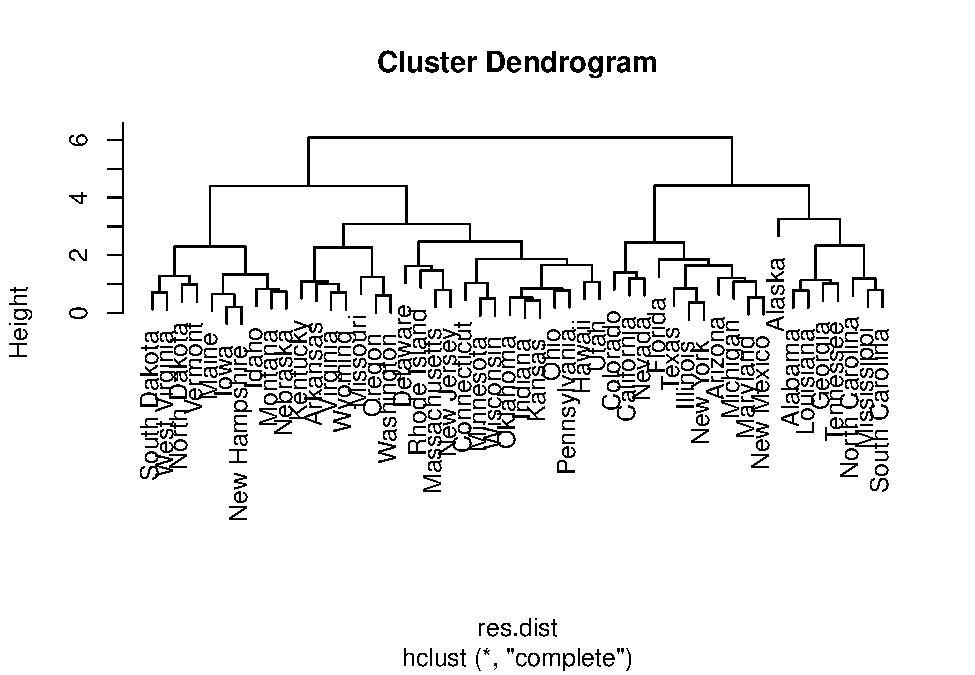
\includegraphics{clusterjerarquico1_files/figure-latex/unnamed-chunk-6-1.pdf}
Otra forma de visualización mejorada del dendrograma es mediante el uso
de factoextrapackage. La función fviz\_dend()dibuja fácilmente
dendrogramas hermosos utilizando la plot()función o ggplot2()función
base R. También proporciona una opción para dibujar un dendrograma
circular y árboles filogénicos.

El x argumento especifica un objeto de la clase dendrogram, hclust,
agnes, diana, hcut, hkmeans o HCPC. El tamaño de las etiquetas y el
ancho de la línea del rectángulo se pueden controlar estableciendo el
valor de cex y lwd como argumentos.

\begin{Shaded}
\begin{Highlighting}[]
\CommentTok{\# Cluster dendrogram using factoextra package}
\FunctionTok{require}\NormalTok{(factoextra)}
\end{Highlighting}
\end{Shaded}

\begin{verbatim}
## Loading required package: factoextra
\end{verbatim}

\begin{verbatim}
## Loading required package: ggplot2
\end{verbatim}

\begin{verbatim}
## Welcome! Want to learn more? See two factoextra-related books at https://goo.gl/ve3WBa
\end{verbatim}

\begin{Shaded}
\begin{Highlighting}[]
\FunctionTok{fviz\_dend}\NormalTok{(}\AttributeTok{x =}\NormalTok{ res.hc, }\AttributeTok{cex =} \FloatTok{0.7}\NormalTok{, }\AttributeTok{lwd =} \FloatTok{0.7}\NormalTok{) }
\end{Highlighting}
\end{Shaded}

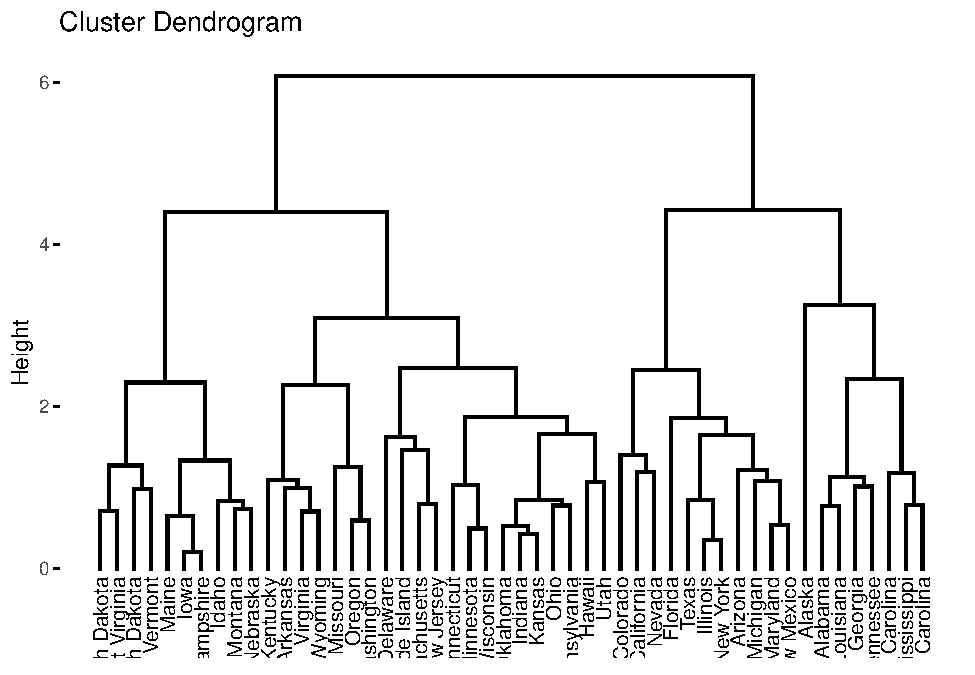
\includegraphics{clusterjerarquico1_files/figure-latex/unnamed-chunk-7-1.pdf}

\hypertarget{personalizar-dendrograma}{%
\subsubsection{Personalizar
dendrograma}\label{personalizar-dendrograma}}

\hypertarget{opciones-de-color}{%
\paragraph{Opciones de color}\label{opciones-de-color}}

Los grupos en el dendrograma se pueden asignar con diferentes nombres de
color integrados en R. La colors()función devuelve los nombres de
colores incorporados que R conoce.

require(grDevices) colors()

Las paletas de gráficos se pueden configurar o visualizar mediante la
palette() función. En R, casi siempre es mejor especificar los colores
por su nombre. La forma rápida de mostrar colores en un gráfico es
mediante la show\_col() función.

\begin{Shaded}
\begin{Highlighting}[]
\FunctionTok{require}\NormalTok{(scales)}
\end{Highlighting}
\end{Shaded}

\begin{verbatim}
## Loading required package: scales
\end{verbatim}

\begin{Shaded}
\begin{Highlighting}[]
\FunctionTok{palette}\NormalTok{()}
\end{Highlighting}
\end{Shaded}

\begin{verbatim}
## [1] "black"   "#DF536B" "#61D04F" "#2297E6" "#28E2E5" "#CD0BBC" "#F5C710"
## [8] "gray62"
\end{verbatim}

\begin{Shaded}
\begin{Highlighting}[]
\FunctionTok{show\_col}\NormalTok{(}\FunctionTok{palette}\NormalTok{(}\FunctionTok{rainbow}\NormalTok{(}\DecValTok{6}\NormalTok{)))}
\end{Highlighting}
\end{Shaded}

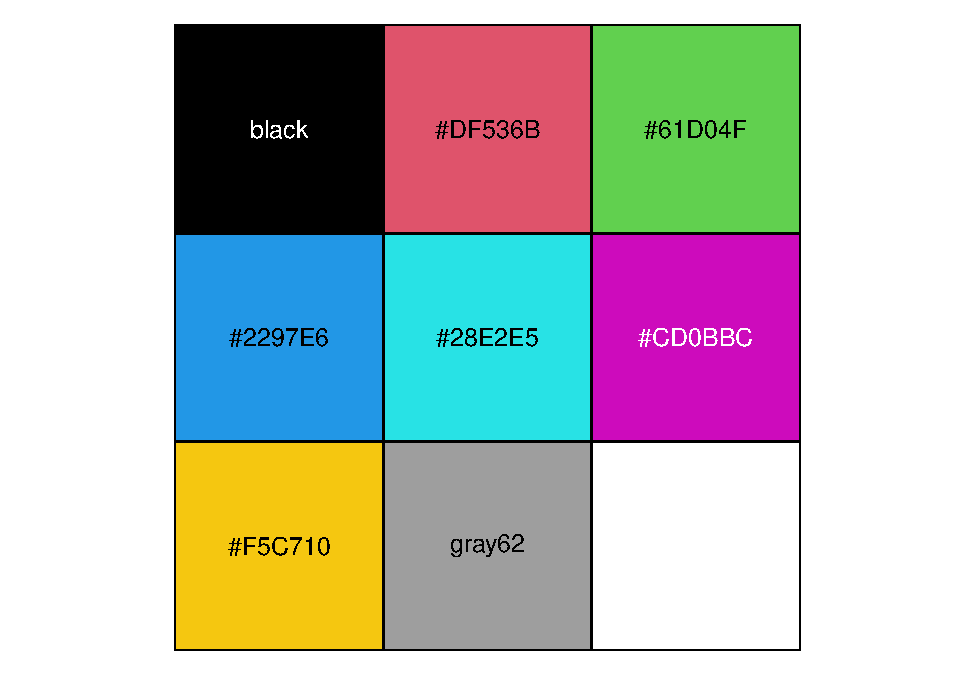
\includegraphics{clusterjerarquico1_files/figure-latex/unnamed-chunk-8-1.pdf}

Para ver las paletas de colores inspiradas en gráficos en la
pal\_jco()función de uso de revista de oncología clínica . El argumento
paletteespecifica el tipo de paleta. Actualmente hay una opción
disponible default(paleta de 10 colores). El argumento alfa especifica
el nivel de transparencia. El valor de este argumento puede estar entre
{[} Error de procesamiento matemático {]}y {[} Error de procesamiento
matemático {]}.

\begin{Shaded}
\begin{Highlighting}[]
\FunctionTok{require}\NormalTok{(}\StringTok{"ggsci"}\NormalTok{)}
\end{Highlighting}
\end{Shaded}

\begin{verbatim}
## Loading required package: ggsci
\end{verbatim}

\begin{Shaded}
\begin{Highlighting}[]
\FunctionTok{show\_col}\NormalTok{(}\FunctionTok{pal\_jco}\NormalTok{(}\AttributeTok{palette =} \FunctionTok{c}\NormalTok{(}\StringTok{"default"}\NormalTok{))(}\DecValTok{10}\NormalTok{))}
\end{Highlighting}
\end{Shaded}

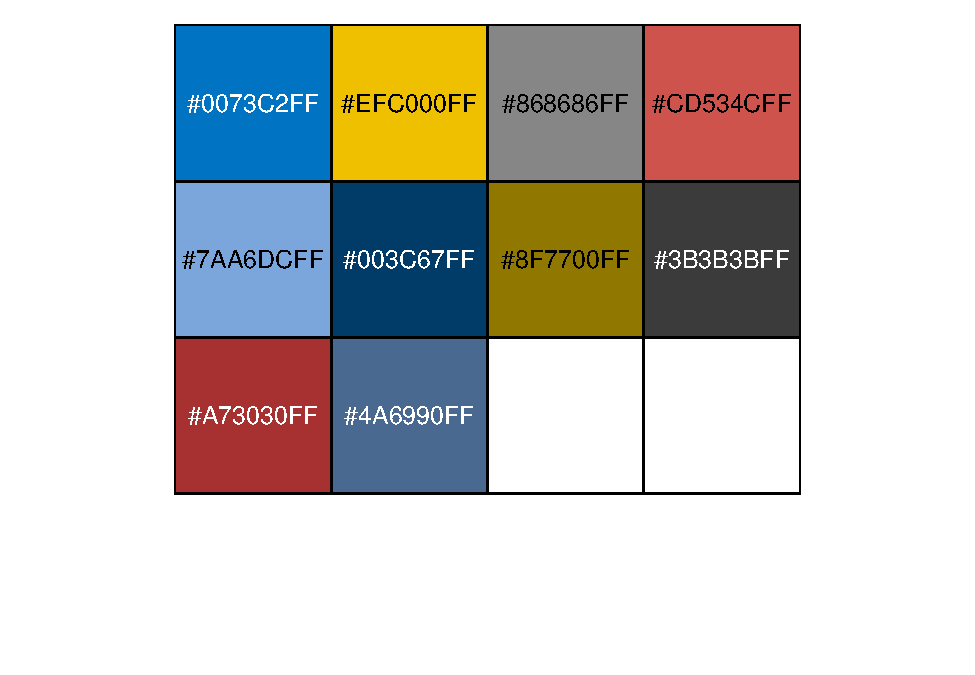
\includegraphics{clusterjerarquico1_files/figure-latex/unnamed-chunk-9-1.pdf}

\begin{Shaded}
\begin{Highlighting}[]
\FunctionTok{show\_col}\NormalTok{(}\FunctionTok{pal\_jco}\NormalTok{(}\StringTok{"default"}\NormalTok{, }\AttributeTok{alpha =} \FloatTok{0.6}\NormalTok{)(}\DecValTok{10}\NormalTok{))}
\end{Highlighting}
\end{Shaded}

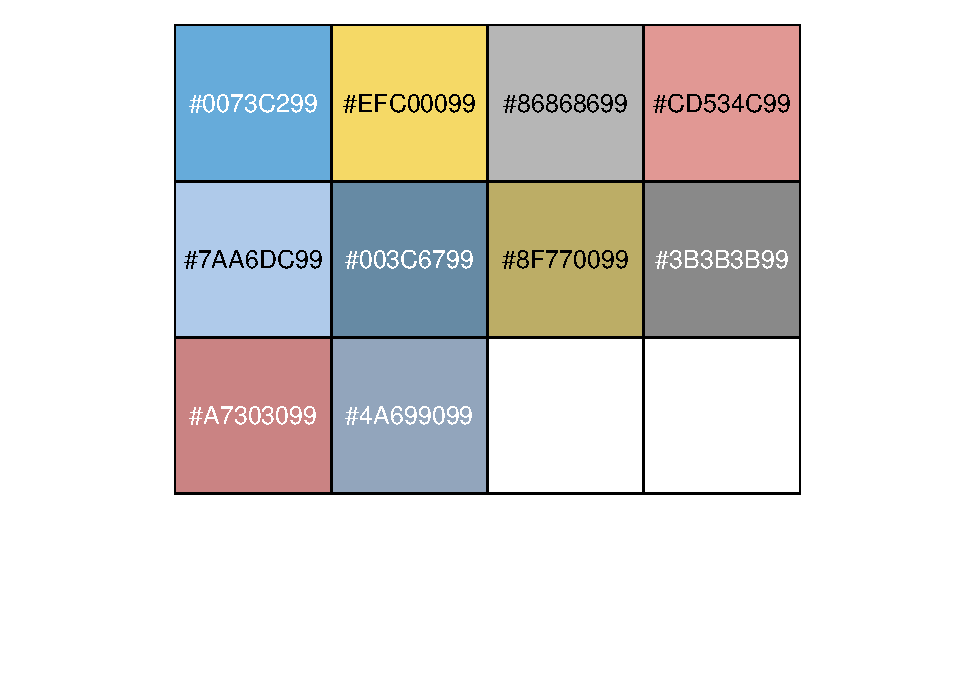
\includegraphics{clusterjerarquico1_files/figure-latex/unnamed-chunk-9-2.pdf}

\hypertarget{asignar-colores-y-dibujar-rectuxe1ngulos}{%
\paragraph{Asignar colores y dibujar
rectángulos}\label{asignar-colores-y-dibujar-rectuxe1ngulos}}

Se pueden agregar colores para el número de grupos o clústeres tanto
para líneas como para rectángulos. El argumento k\_colorsespecifica un
vector que contiene colores que se utilizarán para cada grupo. Los
valores permitidos también incluyen ``gris'' para las paletas de colores
grises; paletas de cerveza y paletas de revistas científicas del paquete
ggsci R.

ggsci: ``Npg'', ``aaas'', ``lancet'', ``jco'', ``ucscgb'', ``uchicago'',
``simpsons'' y ``rickandmorty''

El argumento rectespecifica un valor lógico que indica si se debe
agregar un rectángulo alrededor de los grupos.

Used only when k != NULL.

El color del borde y el tipo de línea de los rectángulos se pueden
personalizar mediante el uso de rect\_border argumentos. El rect\_filles
un argumento lógico si es VERDADERO, llene el rectángulo.

\begin{Shaded}
\begin{Highlighting}[]
\FunctionTok{fviz\_dend}\NormalTok{(}\AttributeTok{x =}\NormalTok{ res.hc, }\AttributeTok{cex =} \FloatTok{0.8}\NormalTok{, }\AttributeTok{lwd =} \FloatTok{0.8}\NormalTok{, }\AttributeTok{k =} \DecValTok{4}\NormalTok{,}
\CommentTok{\# Manually selected colors}
          \AttributeTok{k\_colors =} \FunctionTok{c}\NormalTok{(}\StringTok{"red"}\NormalTok{, }\StringTok{"green3"}\NormalTok{, }\StringTok{"blue"}\NormalTok{, }\StringTok{"magenta"}\NormalTok{),}
          \AttributeTok{rect =} \ConstantTok{TRUE}\NormalTok{, }
          \AttributeTok{rect\_border =} \StringTok{"gray"}\NormalTok{, }
          \AttributeTok{rect\_fill =} \ConstantTok{FALSE}\NormalTok{)}
\end{Highlighting}
\end{Shaded}

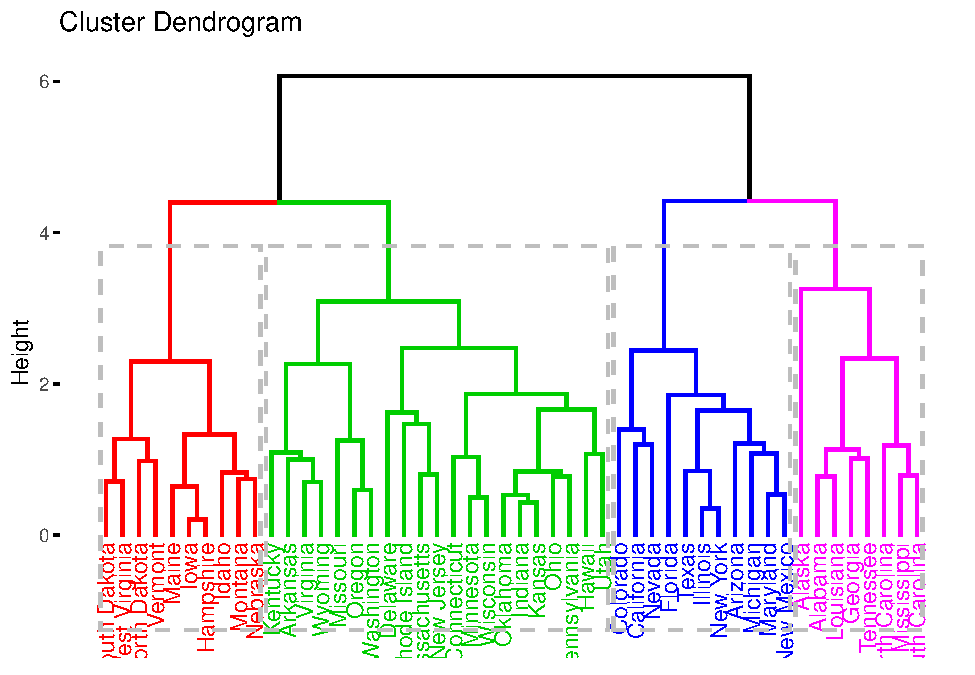
\includegraphics{clusterjerarquico1_files/figure-latex/unnamed-chunk-10-1.pdf}

\begin{Shaded}
\begin{Highlighting}[]
\FunctionTok{fviz\_dend}\NormalTok{(}\AttributeTok{x =}\NormalTok{ res.hc, }\AttributeTok{cex =} \FloatTok{0.8}\NormalTok{, }\AttributeTok{lwd =} \FloatTok{0.8}\NormalTok{, }\AttributeTok{k =} \DecValTok{4}\NormalTok{,}
          

\CommentTok{\# OR JCO fill color for rectangles}
          \AttributeTok{k\_colors =} \FunctionTok{c}\NormalTok{(}\StringTok{"jco"}\NormalTok{),}
          \AttributeTok{rect =} \ConstantTok{TRUE}\NormalTok{, }
          \AttributeTok{rect\_border =} \StringTok{"jco"}\NormalTok{, }
          \AttributeTok{rect\_fill =} \ConstantTok{TRUE}\NormalTok{)}
\end{Highlighting}
\end{Shaded}

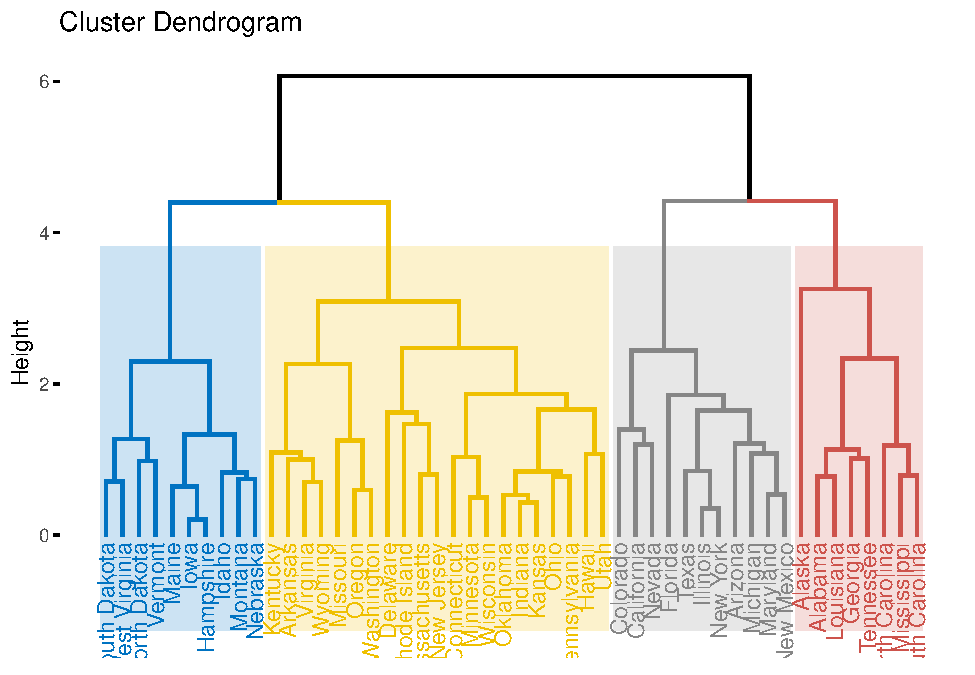
\includegraphics{clusterjerarquico1_files/figure-latex/unnamed-chunk-11-1.pdf}

\hypertarget{alineaciuxf3n-horizontal}{%
\paragraph{Alineación horizontal}\label{alineaciuxf3n-horizontal}}

La alineación del dendrograma se puede cambiar estableciendo un valor
lógico para el horizargumento. La configuración TRUEde este argumento
dibujará un dendrograma horizontal.

\begin{Shaded}
\begin{Highlighting}[]
\FunctionTok{fviz\_dend}\NormalTok{(res.hc, }\AttributeTok{cex =} \FloatTok{0.8}\NormalTok{, }\AttributeTok{k=}\DecValTok{4}\NormalTok{, }
          \AttributeTok{rect =} \ConstantTok{TRUE}\NormalTok{,  }
          \AttributeTok{k\_colors =} \StringTok{"jco"}\NormalTok{,}
          \AttributeTok{rect\_border =} \StringTok{"jco"}\NormalTok{, }
          \AttributeTok{rect\_fill =} \ConstantTok{TRUE}\NormalTok{, }
          \AttributeTok{horiz =} \ConstantTok{TRUE}\NormalTok{)}
\end{Highlighting}
\end{Shaded}

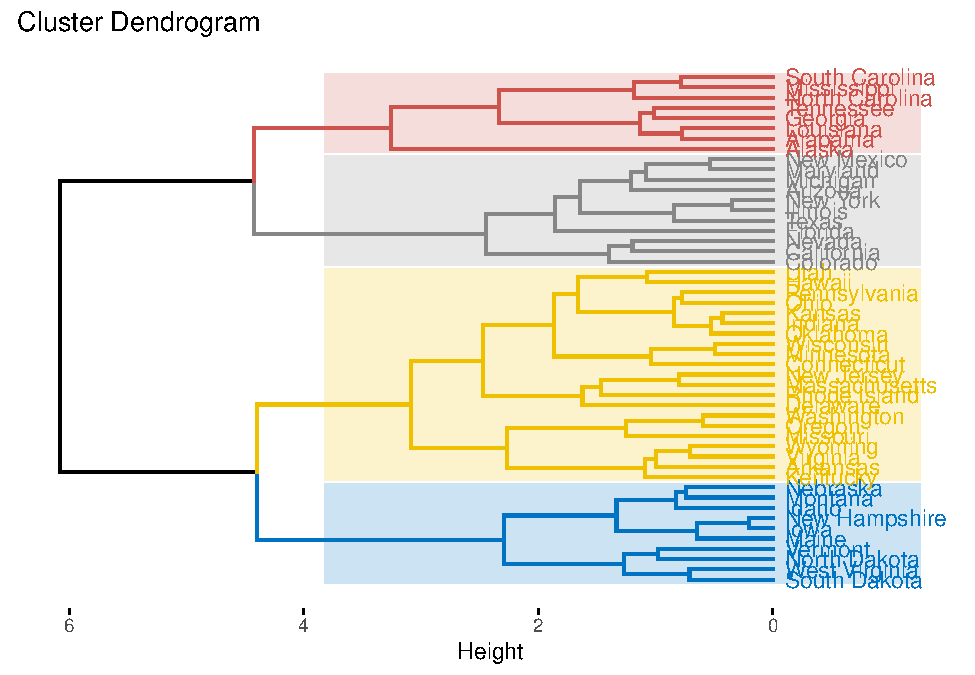
\includegraphics{clusterjerarquico1_files/figure-latex/unnamed-chunk-12-1.pdf}

\hypertarget{aplicar-temas}{%
\paragraph{Aplicar temas}\label{aplicar-temas}}

Se pueden aplicar diferentes temas del paquete ggplot2 al dendrograma
especificando el valor del ggtheme argumento. El valor predeterminado
para este argumento es theme\_classic(). Los valores permitidos para
este argumento incluyen los siguientes temas oficiales de ggplot2 .

ggtheme: theme\_gray (), theme\_bw (), theme\_minimal (), theme\_classic
(), theme\_void (),\ldots.

\begin{Shaded}
\begin{Highlighting}[]
\FunctionTok{fviz\_dend}\NormalTok{(res.hc, }\AttributeTok{cex =} \FloatTok{0.8}\NormalTok{, }\AttributeTok{lwd =} \FloatTok{0.8}\NormalTok{, }\AttributeTok{k =} \DecValTok{4}\NormalTok{, }
          \AttributeTok{rect =} \ConstantTok{TRUE}\NormalTok{, }
          \AttributeTok{k\_colors =} \StringTok{"jco"}\NormalTok{, }
          \AttributeTok{rect\_border =} \StringTok{"jco"}\NormalTok{, }
          \AttributeTok{rect\_fill =} \ConstantTok{TRUE}\NormalTok{,}
          \AttributeTok{ggtheme =} \FunctionTok{theme\_gray}\NormalTok{())}
\end{Highlighting}
\end{Shaded}

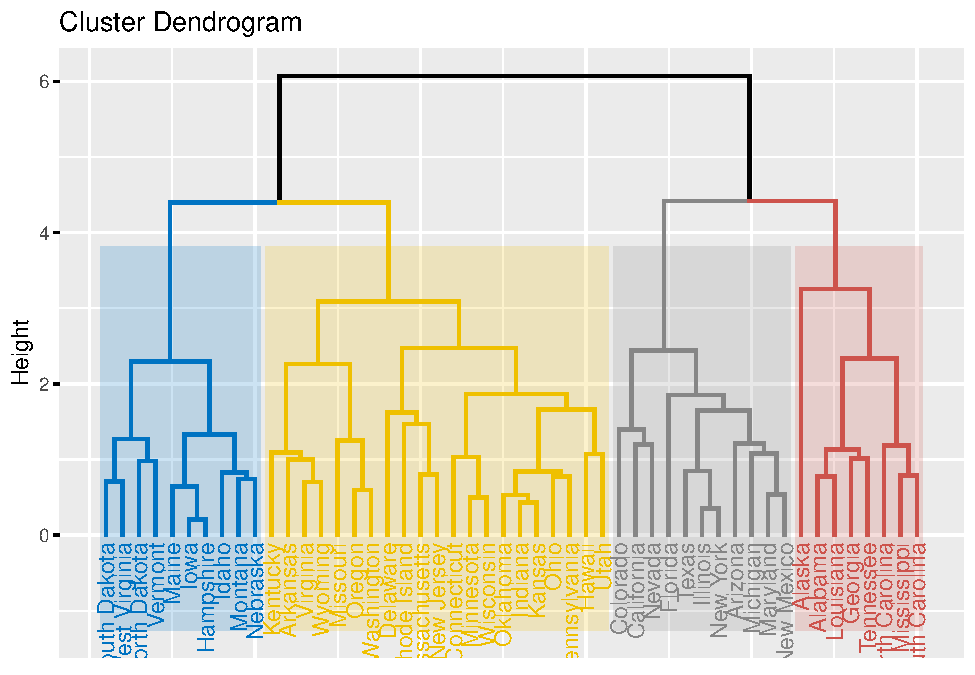
\includegraphics{clusterjerarquico1_files/figure-latex/unnamed-chunk-13-1.pdf}
\#\#\#\# Cambiar el tipo de dendrograma El tipo de dendrograma se puede
cambiar estableciendo un valor para el type argumento. Los valores
permitidos para este argumento son los siguientes:

\begin{Shaded}
\begin{Highlighting}[]
\CommentTok{\#Phylogenic}
\FunctionTok{library}\NormalTok{(igraph)}
\end{Highlighting}
\end{Shaded}

\begin{verbatim}
## 
## Attaching package: 'igraph'
\end{verbatim}

\begin{verbatim}
## The following objects are masked from 'package:stats':
## 
##     decompose, spectrum
\end{verbatim}

\begin{verbatim}
## The following object is masked from 'package:base':
## 
##     union
\end{verbatim}

\begin{Shaded}
\begin{Highlighting}[]
\NormalTok{Phylo }\OtherTok{=} \FunctionTok{fviz\_dend}\NormalTok{(res.hc, }\AttributeTok{cex =} \FloatTok{0.8}\NormalTok{, }\AttributeTok{lwd =} \FloatTok{0.8}\NormalTok{, }\AttributeTok{k =} \DecValTok{4}\NormalTok{,}
                  \AttributeTok{rect =} \ConstantTok{TRUE}\NormalTok{,}
                  \AttributeTok{k\_colors =} \StringTok{"jco"}\NormalTok{,}
                  \AttributeTok{rect\_border =} \StringTok{"jco"}\NormalTok{,}
                  \AttributeTok{rect\_fill =} \ConstantTok{TRUE}\NormalTok{,}
                  \AttributeTok{type =} \StringTok{"phylogenic"}\NormalTok{)}
\NormalTok{Phylo}
\end{Highlighting}
\end{Shaded}

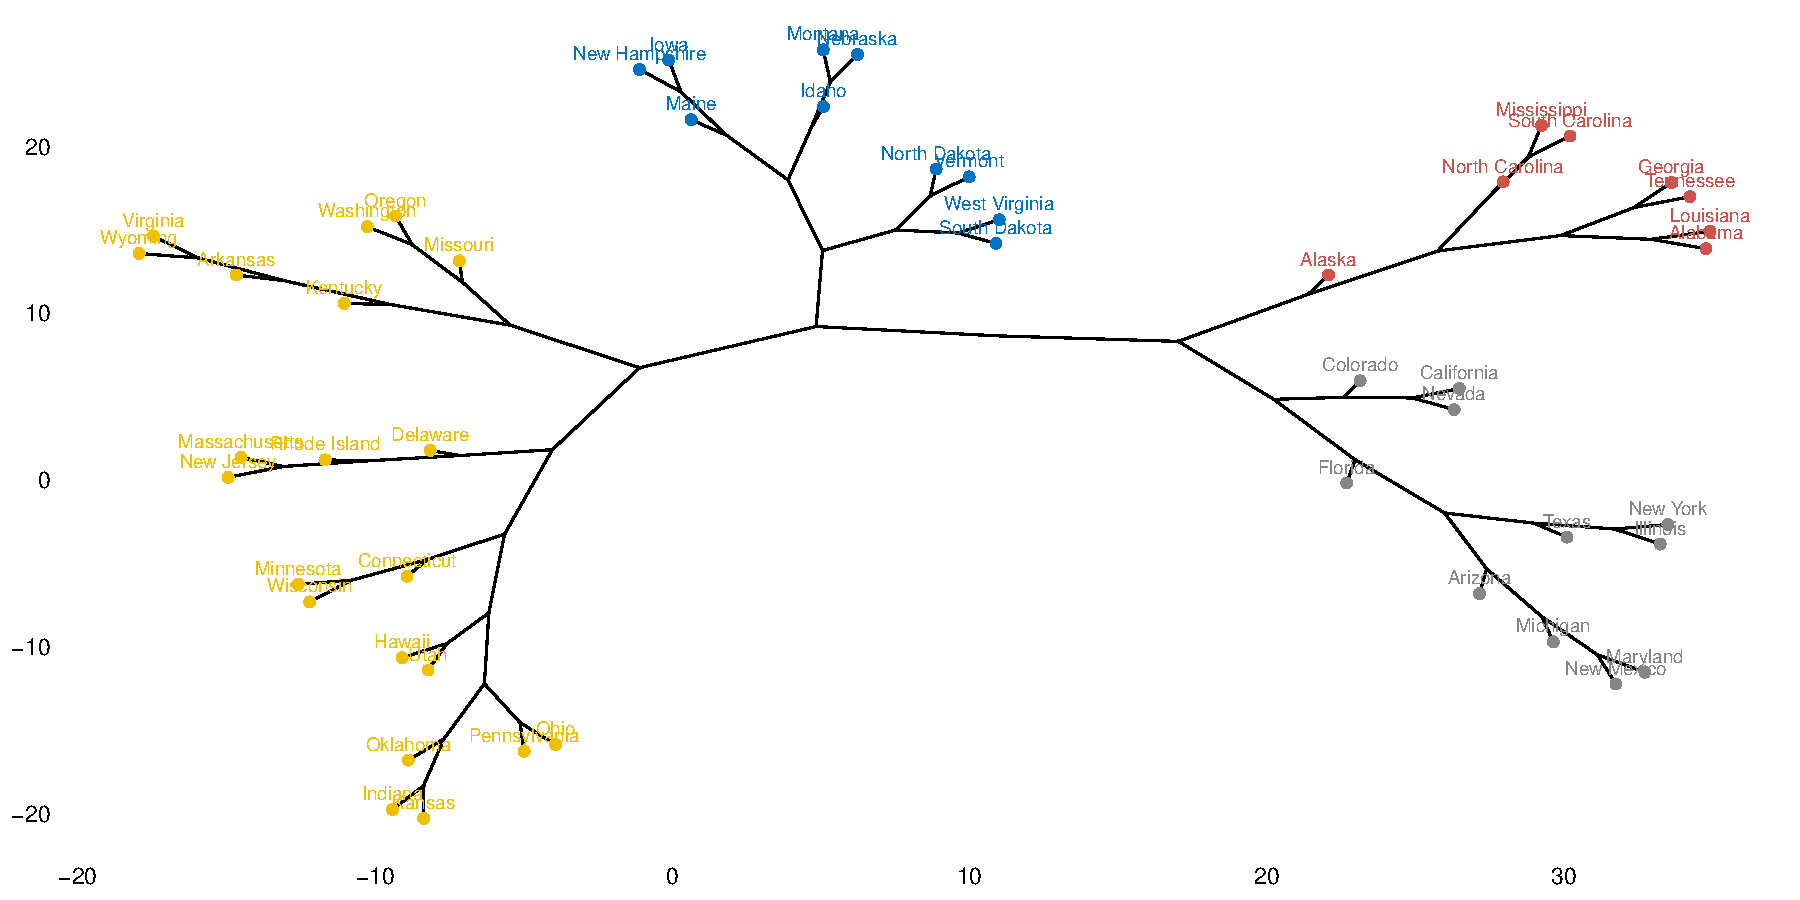
\includegraphics{clusterjerarquico1_files/figure-latex/unnamed-chunk-14-1.pdf}

\begin{Shaded}
\begin{Highlighting}[]
\CommentTok{\# Circular}
\NormalTok{Circ }\OtherTok{=} \FunctionTok{fviz\_dend}\NormalTok{(res.hc, }\AttributeTok{cex =} \FloatTok{0.8}\NormalTok{, }\AttributeTok{lwd =} \FloatTok{0.8}\NormalTok{, }\AttributeTok{k =} \DecValTok{4}\NormalTok{,}
                 \AttributeTok{rect =} \ConstantTok{TRUE}\NormalTok{,}
                 \AttributeTok{k\_colors =} \StringTok{"jco"}\NormalTok{,}
                 \AttributeTok{rect\_border =} \StringTok{"jco"}\NormalTok{,}
                 \AttributeTok{rect\_fill =} \ConstantTok{TRUE}\NormalTok{,}
                 \AttributeTok{type =} \StringTok{"circular"}\NormalTok{)}
\end{Highlighting}
\end{Shaded}

\hypertarget{diseuxf1os-filoguxe9nicos.}{%
\paragraph{Diseños filogénicos.}\label{diseuxf1os-filoguxe9nicos.}}

Se pueden utilizar diferentes diseños para los árboles filogenéticos.
Para hacer esto, establezca un valor para el phylo\_layoutargumento. El
valor predeterminado para este argumento es layout.auto. Los valores
permitidos para este argumento incluyen:

phylo\_layout: ``Layout.auto'', ``layout\_with\_drl'',
``layout\_as\_tree'', ``layout.gem'', ``layout.mds'' y
``layout\_with\_lgl''

\begin{Shaded}
\begin{Highlighting}[]
\FunctionTok{fviz\_dend}\NormalTok{(res.hc, }\AttributeTok{cex =} \FloatTok{0.8}\NormalTok{, }\AttributeTok{lwd =} \FloatTok{0.8}\NormalTok{, }\AttributeTok{k =} \DecValTok{4}\NormalTok{, }
          \AttributeTok{rect =} \ConstantTok{TRUE}\NormalTok{, }\AttributeTok{k\_colors =} \StringTok{"jco"}\NormalTok{, }\AttributeTok{rect\_border =} \StringTok{"jco"}\NormalTok{, }
          \AttributeTok{rect\_fill =} \ConstantTok{TRUE}\NormalTok{, }\AttributeTok{type =} \StringTok{"phylogenic"}\NormalTok{, }\AttributeTok{repel =} \ConstantTok{TRUE}\NormalTok{,}
\CommentTok{\# phylo\_layout (layout\_with\_drl)}
          \AttributeTok{phylo\_layout =} \StringTok{"layout\_with\_drl"}\NormalTok{)}
\end{Highlighting}
\end{Shaded}

\begin{verbatim}
## Warning: ggrepel: 11 unlabeled data points (too many overlaps). Consider
## increasing max.overlaps
\end{verbatim}

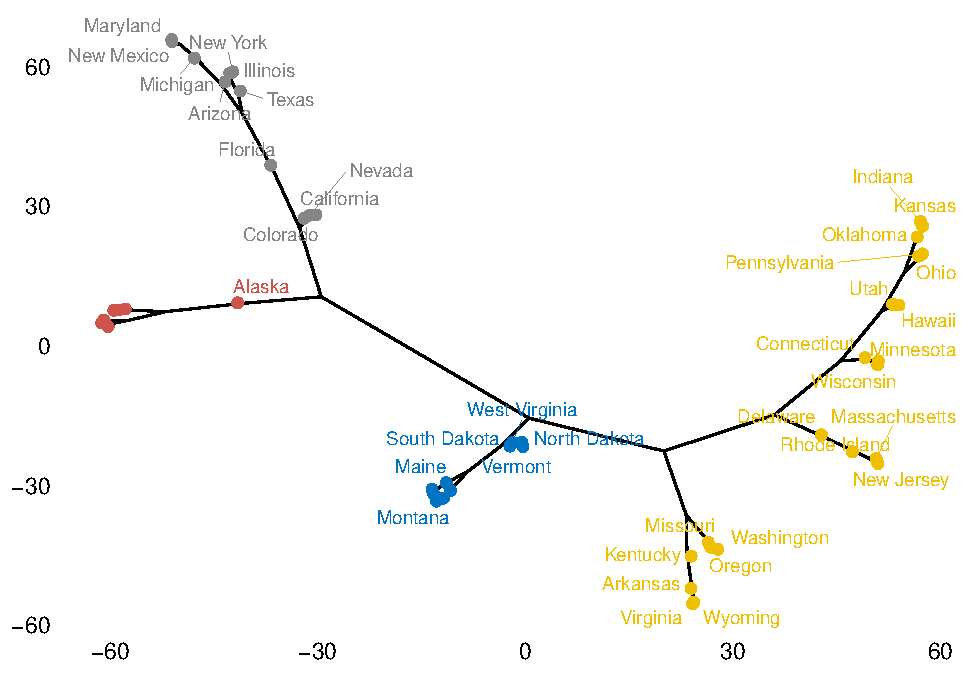
\includegraphics{clusterjerarquico1_files/figure-latex/unnamed-chunk-16-1.pdf}

\begin{Shaded}
\begin{Highlighting}[]
\CommentTok{\# phylo\_layout (layout\_as\_tree)}
          \CommentTok{\#phylo\_layout = "layout\_as\_tree"          }
\CommentTok{\# phylo\_layout (layout.gem)}
          \CommentTok{\#phylo\_layout = "layout.gem"}
\CommentTok{\# phylo\_layout (layout.mds)}
          \CommentTok{\#phylo\_layout = "layout.mds"}
\CommentTok{\# phylo\_layout (layout\_with\_lgl)}
          \CommentTok{\#phylo\_layout = "layout\_with\_lgl"}
\end{Highlighting}
\end{Shaded}


\end{document}
